\documentclass{scrartcl}

\usepackage{amsmath}	  % required for math in general
\usepackage{amsthm}     % environments for theorems, qed's etc
                        % (loaded after amsmath)
\usepackage{amssymb}	  % doublestroke symbols, other mathematical symbols
\usepackage{dsfont}     % required for double-stroke 1 as characteristic function
\usepackage{array}	    % control of matrices and tables
\usepackage{graphicx}   % images

\usepackage{enumitem}   % more fine-grained control over enumerations
\setdescription{leftmargin=\parindent,labelindent=\parindent}

\usepackage{listings} % code listings
\lstset{basicstyle=\ttfamily\scriptsize}

% \input{diagrams.sty} (no category theory this time)

\usepackage{helvet}   % use (much fresher looking) helvetica for everything
\renewcommand{\familydefault}{\sfdefault}

\usepackage[weather]{ifsym}      % \Lightning symbol
% \usepackage{mathabx}             % \Asterisk causes some conflicts

% forcing the fucking floats to stop fucking floating like a fucking piece of
% shit in an ocean of fucking shit
\renewcommand{\topfraction}{.85}
\renewcommand{\bottomfraction}{.7}
\renewcommand{\textfraction}{.15}
\renewcommand{\floatpagefraction}{.66}
\renewcommand{\dbltopfraction}{.66}

% making all references into hyperlinks
\usepackage[dvipsnames]{xcolor}
\usepackage{hyperref}

\hypersetup{colorlinks=true,linkcolor=MidnightBlue,pdfborderstyle={/W 0}}

\usepackage{anyfontsize}
\usepackage{datetime}

% forall
\let\oldforall\forall
\renewcommand{\forall}{\oldforall\,}

% parentheses
\newcommand{\rPar}[1]{\left(#1\right)} % round parens
\newcommand{\sPar}[1]{\left[#1\right]} % square parens
\newcommand{\cPar}[1]{\left\{#1\right\}} % curved parens 
\newcommand{\aPar}[1]{\left\langle #1 \right\rangle} % angle brackets

% floor and ceiling
\newcommand{\floor}[1]{{\left\lfloor#1\right\rfloor}} % curved parens 
\newcommand{\ceil}[1]{{\left\lceil#1\right\rceil}} % curved parens 

% norms
\newcommand{\abs}[1]{\left\lvert #1\right\rvert}
\newcommand{\norm}[1]{\left\lVert #1\right\rVert}
\newcommand{\scalar}[2]{\left\langle#1,#2\right\rangle}
\newcommand{\cross}{\times}
\DeclareMathOperator{\diam}{diam}
\DeclareMathOperator{\B}{B}

% intervals
\newcommand{\openOpenInterval}[2]{{\left(#1,#2\right)}}
\newcommand{\openClosedInterval}[2]{{\left(#1,#2\right]}}
\newcommand{\closedOpenInterval}[2]{{\left[#1,#2\right)}}
\newcommand{\closedClosedInterval}[2]{{\left[#1,#2\right]}}

% restriction of functions
\newcommand{\restrict}[2]{{\left.#1\right\vert_{#2}}}

% numbers
\newcommand{\Natural}{\mathbb{N}}
\newcommand{\Integer}{\mathbb{Z}}
\newcommand{\Real}{\mathbb{R}}
\newcommand{\Rational}{\mathbb{Q}}
\newcommand{\PositiveReal}{\Real_{>0}}
\newcommand{\NonnegativeReal}{\Real_{\geq0}}
\newcommand{\Complex}{\mathbb{C}}
\renewcommand{\i}{i}
\newcommand{\Quaternion}{\mathbb{H}}
\newcommand{\Boolean}{\mathbb{B}}

% function spaces
\newcommand{\SemiLebesgue}{\mathscr{L}}
\newcommand{\Continuous}{C}
\newcommand{\Lebesgue}{L}
\newcommand{\Sobolev}{H}
\newcommand{\Hilbert}{\mathscr{H}}
\newcommand{\Schwarz}{\mathscr{S}}

% set
\newcommand{\setPredicate}[2]{{\left\{#1\,\left\vert\, #2\right.\right\}}}
\newcommand{\set}[1]{{\left\{#1\right\}}}
\newcommand{\cardinality}[1]{\left\lvert #1 \right\rvert}
\newcommand{\powerset}[1]{\mathfrak{P}\left(#1\right)}
\DeclareMathOperator*{\intersection}{\bigcap}
\DeclareMathOperator*{\union}{\bigcup}
\newcommand{\disjointUnion}{\biguplus}
\renewcommand{\complement}[1]{#1^c}
% \newcommand{\setminus}{\backslash}
\newcommand{\injective}{\hookrightarrow}
\newcommand{\surjective}{\twoheadrightarrow}
%\DeclareMathOperator{\ker}{ker} % already exists... im does not?
\DeclareMathOperator{\im}{im}

% topological operators
\DeclareMathOperator{\Cl}{Cl}
\newcommand{\Closure}[2]{\Cl_{#1}\left(#2\right)}
\DeclareMathOperator{\const}{const}

% span and conv
\DeclareMathOperator*{\conv}{conv}
\DeclareMathOperator*{\linhull}{span}

% matrices
\newcommand{\mat}[2]{\left[\begin{array}{#1}#2\end{array}\right]}
\DeclareMathOperator*{\diag}{diag}

% landau symbols
\newcommand{\LandauO}[1]{\mathcal{O}\left(#1\right)}

% derivatives
\newcommand{\dd}[2]{\frac{\partial #1}{\partial #2}}
\newcommand{\differential}[1]{\boldsymbol{D}_{#1}}

% integrals
\renewcommand{\d}{\quad\mathrm{d}}

% characteristic functions, expected values, variances, covariances
% stochastic stuff
\newcommand{\one}[1]{\mathds{1}_{#1}}
\newcommand{\weakconv}[1]{\overset{#1}{\Longrightarrow}}
\newcommand{\wlim}{\mathop{\mathrm{wlim}}}
\newcommand{\vlim}{\mathop{\mathrm{vlim}}}

% lim inf lim sup
% \DeclareMathOperator{\liminf}{lim inf}
% \DeclareMathOperator{\limsup}{lim sup}

% qed etc.
\renewcommand{\qedsymbol}{$\blacksquare$}
\newcommand{\result}{\hfill $\Diamond$}

% lattices
\newcommand{\meet}{\wedge}
\newcommand{\join}{\vee}
\newcommand{\negate}{\neg}

% listings: Scala
\lstdefinelanguage{scala}{
  morekeywords={abstract,case,catch,class,def,%
    do,else,extends,false,final,finally,%
    for,if,implicit,import,match,mixin,%
    new,null,object,override,package,%
    private,protected,requires,return,sealed,%
    super,this,throw,trait,true,try,%
    type,val,var,while,with,yield},
  otherkeywords={=>,<-,<\%,<:,>:,\#,@},
  sensitive=true,
  morecomment=[l]{//},
  morecomment=[n]{/*}{*/},
  morestring=[b]",
  morestring=[b]',
  morestring=[b]"""
}
\lstset{showstringspaces=false}

% making references look a little nices
\let\oldRef\ref
\renewcommand{\ref}[1]{(\oldRef{#1})}

% weird stuff for computer science
\DeclareMathOperator{\arity}{ar}

% cat, category theory
% Bunch of categories
\DeclareMathOperator{\Id}{Id}
\DeclareMathOperator{\Top}{Top}
\DeclareMathOperator{\hTop}{h-Top}
\DeclareMathOperator{\Sets}{Sets}
\DeclareMathOperator{\Rel}{Rel}
\DeclareMathOperator{\FinSets}{FinSets}
\DeclareMathOperator{\Grp}{Grp}
\DeclareMathOperator{\Cat}{Cat}
\DeclareMathOperator{\Grpd}{Grpd}
\newcommand{\cat}[1]{\mathcal{#1}}
\newcommand{\Obj}{\mathrm{Obj}}
\newcommand{\Hom}{\mathrm{Hom}}
\newcommand{\op}{\mathrm{op}}
\newcommand{\nat}{\xrightarrow{\bullet}}
\newcommand{\iso}{\cong}
\newcommand{\dom}{\mathrm{dom}}
\newcommand{\cod}{\mathrm{cod}}
\DeclareMathOperator{\coeq}{Coeq}
\newcommand{\fst}{\mathrm{fst}}
\newcommand{\snd}{\mathrm{snd}}
\DeclareMathOperator{\Aut}{Aut}
\DeclareMathOperator{\End}{End}

% functors frequently used in various contexts
\DeclareMathOperator{\Free}{Free}
\DeclareMathOperator{\Forget}{Forget}

% empty set that is round
\let\emptyset\varnothing

% generated groups
\newcommand{\gen}[1]{\left\langle#1\right\rangle}
\newcommand{\normalSub}{\triangleleft}
\newcommand{\Asterisk}{\mathop{\scalebox{1.5}{\raisebox{-0.2ex}{$\ast$}}}}
\newcommand{\Sym}{\mathrm{Sym}}

% argmax argmin argsup etc.
\DeclareMathOperator{\argsup}{argsup}

% number theoretic operators
\DeclareMathOperator{\lcm}{lcm}

% get rid of the ugly-looking "epsilon"
\renewcommand{\epsilon}{\varepsilon}

% get rid of the empty-looking "angle"
\renewcommand{\angle}{\measuredangle}

\newcommand{\exercise}[2]{\vspace{1em}\noindent{\bf Exercise #1 (#2)}}
\renewcommand{\proof}{\vspace{0.8em}\noindent{\bf Proof: }}

\begin{document}
\noindent{\footnotesize Computer Graphics 2014/15, Exercise 3} 
\hfill 
{\footnotesize \input{./currentDate.txt}}
\newline
{\footnotesize \input{../../NAMES.txt}}

\noindent\hrulefill

\exercise{1.1}{Text with a bunch of funny formulas}

Let $a\in\Real^3$ arbitrary, and let $[a]_\cross$ denote the matrix that
corresponds to the cross product with $a$ from the left:
\[
  [a]_\cross := \mat{ccc}{
    0    & -a_3 & a_1 \\
    a_3  & 0    & -a_2 \\
    -a_1 & a_2  & 0
  }.
\]
It then holds: 
\[
  \exp([a]_\cross) = R_{\frac{a}{\norm{a}}}{\norm{a}},
\]
where $R_{z,\phi}$ is the rotation matrix
around the axis $z$ by the angle $\phi$.

\proof Observe that all powers of $[a]_\cross$ can be 
expressed in terms of $[a]_\cross$ and $[a]_\cross^2$, 
more precisely, it holds (by the Grassmann-Identity):
\begin{align*}
  [a]_\cross^2 &= aa^T - \norm{a}^2I  \\
  [a]_\cross^3 &= -\norm{a}^2[a]_\cross.
\end{align*}
Iteration gives us explicit formulas for all nonnegative powers:
\[
  [a]_\cross^k = \begin{cases}
    I & \textrm{ for } k = 0 \\
    \rPar{(-1)\norm{a}^2}^\frac{k-1}{2}[a]_\cross & \textrm{ for } k \textrm{ odd} \\
    \rPar{-\norm{a}^2}^{\frac{k}{2} - 1}[a]_\cross^2 & 
      \textrm{ for } k \textrm{ even and positive }
  \end{cases}.
\]
Now we start with the series for $\exp$, sort all the terms by 
their matrix-component, and compare the resulting series with $\sin$ and $\cos$:
\begin{align*}
  \exp([a]_\cross) 
    &= \sum_{k=0}^\infty \frac{[a]_\cross^k}{k!}\\
    &= I + \rPar{
         \sum_{k = 1, k \textrm{ odd}}^\infty
         \frac{(-1)^{\frac{k-1}{2}}\norm{a}^{k}}{k!}
       }\sPar{\frac{a}{\norm{a}}}_\cross
       + 
      \rPar{
        \sum_{k = 2, k \textrm{ even}}^\infty
        \frac{-(-1)^\frac{k}{2}\norm{a}^k}{k!}
      }\sPar{\frac{a}{\norm{a}}}_\cross^2 \\
     &= I + \sin(\norm{a})\sPar{\frac{a}{\norm{a}}}_\cross + 
        (1 - \cos(\norm{a}))\sPar{\frac{a}{\norm{a}}}_\cross^2.
\end{align*}
We have already shown that the last expression is exactly the 
rotation matrix $R_{\frac{a}{\norm{a}}}{\norm{a}}$, 
this concludes the proof.  \hfill\qed

\exercise{1.2}{A funny image}
Here you can see an example of an image.
\begin{figure}[htbp]
  \centering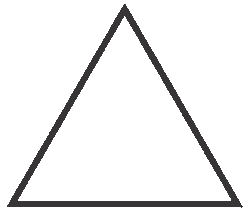
\includegraphics[width=0.5\linewidth]{images/exampleImage.png}
\end{figure}
And here is some more text:
\begin{align*}
  [a]_\cross^2 &= aa^T - \norm{a}^2I  \\
  [a]_\cross^3 &= -\norm{a}^2[a]_\cross.
\end{align*}
Iteration gives us similar expressions for all positive powers:
\[
  [a]_\cross^k = \begin{cases}
    I & \textrm{ for } k = 0 \\
    \rPar{(-1)\norm{a}^2}^\frac{k-1}{2}[a]_\cross & \textrm{ for } k \textrm{ odd} \\
    \rPar{-\norm{a}^2}^{\frac{k}{2} - 1}[a]_\cross^2 & 
      \textrm{ for } k \textrm{ even and positive }
  \end{cases}.
\]
Now we start with the series for $\exp$, sort all the terms by 
their matrix-component, and compare the resulting series with $\sin$ and $\cos$:
\begin{align*}
  \exp([a]_\cross) 
    &= \sum_{k=0}^\infty \frac{[a]_\cross^k}{k!}\\
    &= I + \rPar{
         \sum_{k = 1, k \textrm{ odd}}^\infty
         \frac{(-1)^{\frac{k-1}{2}}\norm{a}^{k}}{k!}
       }\sPar{\frac{a}{\norm{a}}}_\cross
       + 
      \rPar{
        \sum_{k = 2, k \textrm{ even}}^\infty
        \frac{-(-1)^\frac{k}{2}\norm{a}^k}{k!}
      }\sPar{\frac{a}{\norm{a}}}_\cross^2 \\
     &= I + \sin(\norm{a})\sPar{\frac{a}{\norm{a}}}_\cross + 
        (1 - \cos(\norm{a}))\sPar{\frac{a}{\norm{a}}}_\cross^2.
\end{align*}
Blah blah blah...

\exercise{1.3}{Code-examples}
Here is how one can include formatted code:
\begin{lstlisting}
  ...
  void main(void) {
    cout << "blah";
  }
\end{lstlisting}
You might also find \verb|\lstinputlisting[firstline=n,lastline=m]| useful.
\end{document}
